\section{实验}
\label{sec:experiments}

我们围绕三个问题组织实证研究：AHE 在既有 harness 设计方法的版图中处于什么位置；它产出的成果能否迁移到其优化目标之外；以及闭环内部究竟是什么在驱动收益。

\begin{tcolorbox}[
    colback=blue!3,
    colframe=blue!40,
    arc=2pt,
    boxrule=0.5pt,
    left=6pt, right=6pt, top=4pt, bottom=4pt,
    title={\textbf{研究问题}},
    fonttitle=\bfseries,
    coltitle=black,
    colbacktitle=blue!10
  ]
  \begin{enumerate}
    \setlength{\leftmargini}{1.5em}
    \setlength{\itemsep}{2pt}
    \setlength{\parsep}{0pt}
      \item \textbf{RQ1}（\S\ref{sec:experiments:main}）\textbf{：为什么要做 agentic harness engineering，而不是采用人工设计的 harness 或其他自动化方法？}
      \item \textbf{RQ2}（\S\ref{sec:experiments:transfer}）\textbf{：agentic harness engineering 是否会过拟合到它的优化目标上？}
      \item \textbf{RQ3}（\S\ref{sec:experiments:mechanism}）\textbf{：AHE 内部是什么在驱动收益，闭环的自归因又有多可靠？}
  \end{enumerate}
\end{tcolorbox}

\subsection{实验设置}
\label{sec:experiments:setup}

\paragraph{评测。}
\label{sec:experiments:metrics}
我们在 Terminal-Bench 2~\citep{merrillTerminalBenchBenchmarkingAgents2026a} 的全部 89 个任务上驱动演化，其难度划分为 4 个 easy、55 个 medium 和 30 个 hard，并将单任务超时延长至 1 小时。对于跨基准的迁移，我们在 SWE-bench-verified~\citep{jimenezSWEbenchCanLanguage2023} 上评测 AHE harness，该基准包含跨七个代码仓库的 500 个任务。
我们为每个配置报告两项指标：\textit{pass@1}，即每个任务 $k$ 次 rollout 上二值成功率的均值；以及 \textit{tokens/trial}，即所有 LLM 调用的提示词 token 与补全 token 之和在每次试验上的均值，以千为单位。因基础设施中止或超时的试验在 pass@1 下计为失败（与官方 terminal-bench 排行榜的口径一致），并从 token 均值中剔除，以免得到被截断的数值。运行时基础设施（框架、调度器、沙箱、追踪器与并发设置）详见附录~\ref{app:setup}。

\paragraph{模型。}
在演化闭环与 \S\ref{sec:experiments:main} 的主实验中，三个角色智能体（Code Agent、Agent Debugger 与 Evolve Agent）共享同一个基座模型：GPT-5.4~\citep{openaiIntroducingGPT542026}，推理档位为 high。
% Fixing the model across roles isolates the effect of harness edits from confounds introduced by a different analyzer or editor.
对于跨模型迁移（\S\ref{sec:experiments:transfer}），我们在五个替代基座上重新评测 Code Agent：medium 与 xhigh 推理档位的 GPT-5.4~\citep{openaiIntroducingGPT542026}、qwen-3.6-plus~\citep{teamQwen36PlusRealWorld2026,yangQwen3TechnicalReport2025a}、gemini-3.1-flash-lite-preview~\citep{googleGemini31FlashLiteModelCard2026} 以及 deepseek-v4-flash~\citep{DeepSeek_V4pdfDeepseekaiDeepSeekV4Pro2026}。

\subsection{RQ1：主要结果}
\label{sec:experiments:main}

% \input{figures/evolution-curve}

\input{tables/main-results_zh}
我们在 Terminal-Bench 2 上从仅含 bash 的 \textbf{NexAU\textsubscript{0}} 种子（\S\ref{sec:method:harness}）出发，运行了一次共十轮迭代的 AHE 演化，历时约 32 小时；其中最优配置被报告为 \textbf{AHE}。两个自演化基线 ACE~\citep{zhangAgenticContextEngineering2025a} 与 Training-Free GRPO（TF-GRPO）~\citep{caiTrainingFreeGroupRelative2025} 也从同一个 NexAU\textsubscript{0} 种子出发。

\paragraph{AHE 同时超越人工设计的与自演化的基线。}
AHE 在我们的对照面板上超越了每一个基线：三个人工设计的 harness——OpenCode~\citep{anomalyOpencodeOpenSource2025}、Terminus-2~\citep{harborTerminus22026} 与 Codex~\citep{openaiCodexCLI2025}，以及两个自演化基线。
图~\ref{fig:training_curve} 显示收益是跨迭代累积的，持续演化把 pass@1 进一步推高到 NexAU\textsubscript{0} 种子之上。
按难度看，唯一的例外是 Hard 档，AHE 在该档略微落后于 Codex。我们把这一差距归因于 AHE 各组件在长程任务上的相互干扰，而非缺失某项能力：只把 AHE 的长期记忆单独换入 NexAU\textsubscript{0} 种子、不引入其他 AHE 组件，就已经在 Hard 上超过了 Codex（\S\ref{sec:experiments:rq3a}）。

\paragraph{仅提示词的自演化错过了承载 AHE 收益的那些组件。}
与 ACE 和 TF-GRPO 的差距源于层次上的错配。ACE 蒸馏出智能体在上下文中阅读的自然语言操作手册，而 TF-GRPO 是 GRPO 的一种轨迹反馈变体，用于强化成功的工具调用序列；两种方法都没有把外围脚手架开放给编辑。
AHE 则联合演化系统提示词、工具、中间件与长期记忆，而 \S\ref{sec:experiments:rq3a} 表明收益集中在后三个组件上，恰恰是 ACE 与 TF-GRPO 未曾触及的层次。

\subsection{RQ2：向未见任务与基座模型的迁移}
\label{sec:experiments:transfer}

AHE 的 harness 是在 Terminal-Bench 2 上以 GPT-5.4 high 演化得到的。我们把演化后的 harness 原封不动、不再继续演化地迁移到两类目标外设置中，以检验它编码的是通用的 coding agent 经验，还是对该目标的过拟合：一个不同的任务面（SWE-bench-verified）以及三个替代基座模型。

\begin{table}[t]
    \centering
    \small
    \setlength{\tabcolsep}{5pt}
    \renewcommand{\arraystretch}{1.05}
    \caption{SWE-bench-verified 上的跨基准迁移。ACE、Training-Free GRPO（TF-GRPO）与 \textbf{AHE} 共享 \textbf{NexAU\textsubscript{0}} 种子，仅在各自的自演化闭环上不同；四列全部运行在 GPT-5.4 上。AHE 与两个自演化基线都是在 Terminal-Bench 2 上演化得到的，评测时不做域内再演化。每列粗体标出最优；并列时全部加粗。}
    \label{tab:swe-verified-analysis}
    \begin{tabular}{lc @{\hspace{10pt}} cccc @{\hspace{10pt}} cccc}
        \toprule
         &  & \multicolumn{4}{c}{成功率 $\uparrow$} & \multicolumn{4}{c}{Tokens k $\downarrow$} \\
        \cmidrule(lr){3-6} \cmidrule(lr){7-10}
        仓库 & $N$
        & ACE & TF-GRPO & NexAU\textsubscript{0} & \textbf{AHE}
        & ACE & TF-GRPO & NexAU\textsubscript{0} & \textbf{AHE} \\
        \midrule
        全部            & 500 & 74.6\% & 74.2\% & 75.2\% & \textbf{75.6\%} & 679 & 582 & 526 & \textbf{461} \\
        \midrule
        django         & 231 & 79.2\% & 78.8\% & 79.2\% & \textbf{81.0\%} & 707 & 583 & 527 & \textbf{484} \\
        sympy          &  75 & 69.3\% & 68.0\% & \textbf{70.7\%} & \textbf{70.7\%} & 602 & 572 & 494 & \textbf{479} \\
        sphinx-doc     &  44 & 61.4\% & 65.9\% & 68.2\% & \textbf{70.5\%} & 990 & 848 & 731 & \textbf{656} \\
        matplotlib     &  34 & 70.6\% & 70.6\% & \textbf{73.5\%} & \textbf{73.5\%} & 622 & 530 & 486 & \textbf{391} \\
        scikit-learn   &  32 & \textbf{93.8\%} & \textbf{93.8\%} & \textbf{93.8\%} & 87.5\% & 451 & 378 & 307 & \textbf{257} \\
        pydata         &  22 & \textbf{77.3\%} & \textbf{77.3\%} & \textbf{77.3\%} & 72.7\% & 563 & 516 & 386 & \textbf{338} \\
        astropy        &  22 & \textbf{59.1\%} & \textbf{59.1\%} & 54.5\% & 50.0\% & 546 & 470 & 667 & \textbf{277} \\
        \bottomrule
    \end{tabular}
\end{table}


\paragraph{跨基准迁移。}
我们在完全相同的基础设施下，于 SWE-bench-verified 上把 AHE harness 与种子及两个自演化基线（NexAU\textsubscript{0}、ACE、TF-GRPO）进行对比评测（表~\ref{tab:swe-verified-analysis}）。

ACE 与 TF-GRPO 在总体成功率上都跌到 NexAU\textsubscript{0} 种子之下，同时比种子多消耗 $11\%$ 到 $29\%$ 的 token：ACE 注入的操作手册与 TF-GRPO 强化的轨迹分布，都是在 Terminal-Bench 2 的轨迹上蒸馏出来的，并且在每一次模型调用时都随提示词一同带入，因此在不同的任务面上，这些文本只增加了成本，却没有重塑底层策略。

AHE 则取得了最高的总体成绩，相对种子的增益集中在 django 与 sphinx-doc 这两个规模最大、token 开销最高的仓库上——它们的多步「编辑—验证」循环，正好与 AHE 的工具、中间件和长期记忆在 Terminal-Bench 2 上所压缩的结构相吻合。
轻微的回归只出现在三个最小的仓库上，这与小仓库上 pass@1 的方差超过其单仓库增益的情形一致。
AHE 还把总体 token 消耗相对 ACE 削减了 $32\%$、相对 TF-GRPO 削减了 $21\%$、相对种子削减了 $12\%$：把行为编码进工具、中间件与记忆之中，避免了仅提示词的基线所付出的逐次调用重新推导成本。

\begin{figure}[t]
    \centering
    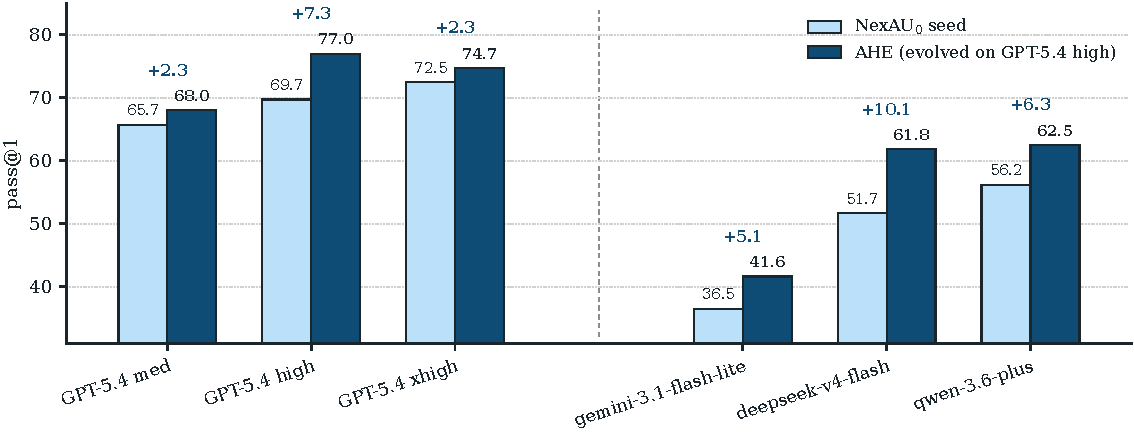
\includegraphics[width=0.9\linewidth]{figures/transfer_model.pdf}
    \caption{Terminal-Bench 2 上 89 个任务的跨模型迁移。在 GPT-5.4 high 上演化得到的 AHE 工作区在每个底座模型上重新评测，不做进一步演化，并与同一底座上的 NexAU\textsubscript{0} 种子配对比较。所有底座相对种子都有提升，其中跨家族底座的提升大于同家族底座。}
    \label{fig:transfer-model}
\end{figure}


\paragraph{跨模型迁移。}
我们在 \S\ref{sec:experiments:setup} 列出的五个替代基座上，对 NexAU\textsubscript{0} 种子与 AHE 分别重新评测。图~\ref{fig:transfer-model} 报告了从 $+2.3$ 到 $+10.1$\,个百分点的五个正向 pass@1 增益。

跨模型家族的增益明显大于同家族内部的增益：deepseek-v4-flash 从 $51.7\%$ 提升到 $61.8\%$，增幅 $+10.1$\,个百分点；qwen-3.6-plus 从 $56.2\%$ 提升到 $62.5\%$，增幅 $+6.3$\,个百分点；gemini-3.1-flash-lite-preview 从 $36.5\%$ 提升到 $41.6\%$，增幅 $+5.1$\,个百分点；三者都高于 GPT-5.4 medium 与 xhigh 上的 $+2.3$\,个百分点。我们对此的解读是：离饱和更远的基座更依赖 AHE 已固化在工具、中间件与长期记忆中的协同模式，而更强的基座能以很低的边际成本从自身提示词中重新推导出同样的协同。

在同一家族内部，其表现是非单调的：medium 上 $+2.3$\,个百分点，high 上（来自 \S\ref{sec:experiments:main}）$+7.3$\,个百分点，xhigh 上 $+2.3$\,个百分点。AHE 的步数预算与单任务超时是在演化过程中针对 GPT-5.4 high 拟合的；medium 每一步的时间余量更充裕，但在原始能力上损失了一个推理档位，而 xhigh 则使更多试验超出单任务超时，按我们的 pass@1 约定（\S\ref{sec:experiments:metrics}）这些都计为失败。两个方向都会削减增益。

最重要的发现是五个增益全部为正：AHE 工作区并不专属于某一家供应商的惯用范式或某一种推理深度。增益的幅度跟随的是演化的工作点，而非基座的原始能力，因此我们把这种超时—预算耦合视为一种泛化风险，并在 \nameref{sec:limitations} 一节中加以讨论。

\subsection{RQ3：分析}
\label{sec:experiments:mechanism}

我们沿着 \S\ref{sec:method} 所强调的两个架构选择来分析这一闭环：分解式组件（\S\ref{sec:experiments:rq3a}）与自我声明的归因（\S\ref{sec:experiments:rq3b}）。


\subsubsection{RQ3a：价值累积在哪些组件上}
\label{sec:experiments:rq3a}


表~\ref{tab:ablations} 在组件层面分解了 AHE 的收益：每次只隔离出四个被演化层之一——长期记忆、工具、中间件或系统提示词，同时把其余三层保持在种子的默认状态。四个单组件变体中有三个优于种子；只有替换系统提示词这一项出现了回归。

\begin{table}[htbp]
    \centering
    \small
     \vspace{\baselineskip}
    \caption{Terminal-Bench 2 上的组件级消融。每一行``+\,X only''把单个 AHE 组件换入 NexAU\textsubscript{0} 种子；每列最优值以粗体标出。多数单组件替换已经超过种子，且各单组件增益之和超过了完整 AHE 的总增益，说明各组件之间是非可加地相互作用，而非干净地叠加。}
    \label{tab:ablations}
    \begin{tabular}{lcccc}
        \toprule
        变体 & 全部 & 简单 & 中等 & 困难 \\
                & {\scriptsize 89 个任务} & {\scriptsize 4 个任务} & {\scriptsize 55 个任务} & {\scriptsize 30 个任务} \\
        \midrule
        NexAU\textsubscript{0} & 69.7\% & 87.5\% & 78.2\% & 51.7\% \\
        \addlinespace
        + 仅长期记忆         & 75.3\% & 50.0\% & 83.6\% & \textbf{63.3\%} \\
        + 仅工具           & 73.0\% & 75.0\% & 87.3\% & 46.7\% \\
        + 仅中间件     & 71.9\% & \textbf{100.0\%} & 81.8\% & 50.0\% \\
        + 仅 system\_prompt & 67.4\% & 75.0\% & 78.2\% & 46.7\% \\
        \addlinespace
        \textbf{AHE} 完整     & \textbf{77.0\%} & \textbf{100.0\%} & \textbf{88.2\%} & 53.3\% \\
        \bottomrule
    \end{tabular}
\end{table}


\paragraph{每个组件各自负责一类不同的失败面。}
记忆增加了 12 条边界情形的经验教训（性能余量、超限排队时的取消、evaluator 风格的收尾、源码打包布局）；在 Hard 档上这些教训使其超过完整的 AHE，而在 Easy 档上它们退化为多余的重复验证。
工具演化成了一个 1364 行的 shell，可从每条命令附近的文件中自动浮现契约提示；在 Medium 档上它与完整 AHE 的差距在 $0.9$\,个百分点以内，而在 Hard 档上其内置的发布守卫会过早地关闭循环。
中间件加入了一个 finish 钩子，强制执行一次与 evaluator 同构的收尾检查；在 Easy 档上它通过了每一个任务，而在 Hard 档上它抬高了轮次数量。
系统提示词编码了 79 行通用纪律，其可执行性依赖于其余三个组件；单独插入时其总体成绩为 $-2.3$\,个百分点。

\paragraph{各组件之间以非可加的方式相互作用，从而给总体收益设了上限。}
三个为正的单组件增益加总为 $+11.1$\,个百分点，而完整 AHE 只有 $+7.3$\,个百分点，并且在 Hard 档上仅含记忆的变体超过了完整 AHE：记忆、中间件与系统提示词都在推动同一种收尾式的验证，因此把它们叠加起来，会在长程任务的预算内把轮次花在冗余的重复检查上。
由于 Evolve Agent 优化的是一个由 55 个 Medium 任务主导的总体指标，它收敛到了一个偏向 Medium 的权衡，从而让出了一部分 Hard 档上的记忆效应；我们把考虑组件交互的演化留作未来工作。

\subsubsection{RQ3b：闭环的自归因在多大程度上贴合现实}
\label{sec:experiments:rq3b}

在每一轮演化中，我们的演化模型都会产出一份变更清单，指明它预期在下一轮中修复哪些 Terminal-Bench 2 任务，以及它标记出哪些任务有回归风险。我们把第 $N{-}1$ 轮的预测与第 $N$ 轮的真实结果进行比较，在 89 个任务上分别针对修复与回归计算标准的精确率与召回率。

\paragraph{证据驱动的目标定位。}
\Cref{fig:pred-aggregate} 的修复面板表明，演化模型的目标定位是证据驱动的，而非凭空猜测。跨迭代的修复精确率为 \textbf{33.7\%}、修复召回率为 \textbf{51.4\%}，大约是随机预测基线 6.5\% 与 10.6\% 的 5 倍，因此每一次 harness 编辑都落在一个真实且被智能体预期到的目标上，而不是落在面板中任意的一个子集上。

\begin{figure}[t]
    \centering
    \begin{minipage}{0.4\linewidth}
        \centering
        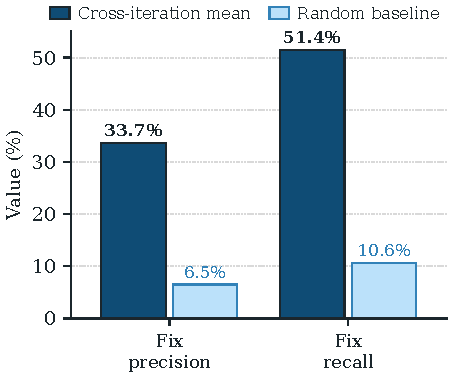
\includegraphics[width=\linewidth]{figures/summary_fix.pdf}
    \end{minipage}
    % \hfill
    \begin{minipage}{0.4\linewidth}
        \centering
        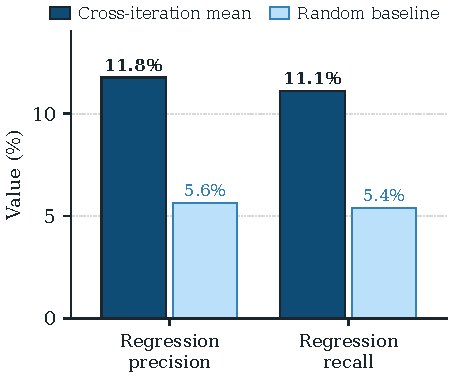
\includegraphics[width=\linewidth]{figures/summary_regression.pdf}
    \end{minipage}
    \caption{在 Terminal-Bench 2 上运行的 GPT-5.4 AHE 闭环的 9 个评测轮次中，演化模型自我预测的跨迭代平均精确率与召回率，并与随机预测基线对照。左：修复预测。右：回归预测。}
    \label{fig:pred-aggregate}
\end{figure}

\paragraph{回归盲区。}
回归面板讲述的却是相反的故事：跨迭代的回归精确率为 \textbf{11.8\%}、回归召回率为 \textbf{11.1\%}，仅约为其随机基线 5.6\% 与 5.4\% 的 2 倍，因此大多数即将发生的回归都未被预见。智能体能够论证某次编辑为何应当有帮助，却无法可靠地指出同一次编辑即将破坏哪些任务，而这正是 \S\ref{sec:experiments:main} 中演化曲线出现非单调台阶的原因。弥合这一差距是未来自演化闭环最明确的方向。附录~\ref{sec:appendix:self-attribution} 给出了逐轮的细分结果。
